\documentclass{article}

\usepackage[T1]{fontenc}
\usepackage{fancyhdr} % Required for custom headers
\usepackage{lastpage} % Required to determine the last page for the footer
\usepackage{extramarks} % Required for headers and footers
\usepackage[usenames,dvipsnames]{color} % Required for custom colors
\usepackage{graphicx} % Required to insert images
\usepackage{listings} % Required for insertion of code
\usepackage{courier} % Required for the courier font
\usepackage{lipsum} % Used for inserting dummy 'Lorem ipsum' text into the template
\usepackage{hyperref}
\usepackage{color}
\usepackage[normalem]{ulem}
\usepackage{url}

% Margins
\topmargin=-0.45in
\evensidemargin=0in
\oddsidemargin=0in
\textwidth=6.5in
\textheight=9.0in
\headsep=0.25in

\linespread{1.1} % Line spacing

% Set up the header and footer
\pagestyle{fancy}
\lhead{\hmwkAuthorName} % Top left header
\chead{\hmwkClass\ (\hmwkClassInstructor): \hmwkTitle} % Top center head
\rhead{\firstxmark} % Top right header
\lfoot{\lastxmark} % Bottom left footer
\cfoot{} % Bottom center footer
\rfoot{Page\ \thepage\ of\ \protect\pageref{LastPage}} % Bottom right footer
\renewcommand\headrulewidth{0.4pt} % Size of the header rule
\renewcommand\footrulewidth{0.4pt} % Size of the footer rule

\setlength\parindent{0pt} % Removes all indentation from paragraphs

\usepackage{listings}
\usepackage{color}

\definecolor{dkgreen}{rgb}{0,0.6,0}
\definecolor{gray}{rgb}{0.5,0.5,0.5}
\definecolor{mauve}{rgb}{0.58,0,0.82}

\lstset{frame=tb,
  language=Java,
  aboveskip=3mm,
  belowskip=3mm,
  showstringspaces=false,
  columns=flexible,
  basicstyle={\small\ttfamily},
  numbers=none,
  numberstyle=\tiny\color{gray},
  keywordstyle=\color{blue},
  commentstyle=\color{dkgreen},
  stringstyle=\color{mauve},
  breaklines=true,
  breakatwhitespace=true
  tabsize=3
}

\DeclareUrlCommand\ULurl{%
  \renewcommand\UrlFont{\ttfamily\color{blue}}%
  \renewcommand\UrlLeft{\uline\bgroup}%
  \renewcommand\UrlRight{\egroup}}



%----------------------------------------------------------------------------------------
%	DOCUMENT STRUCTURE COMMANDS
%	Skip this unless you know what you're doing
%----------------------------------------------------------------------------------------

% Header and footer for when a page split occurs within a problem environment
\newcommand{\enterProblemHeader}[1]{
\nobreak\extramarks{#1}{#1 continued on next page\ldots}\nobreak
\nobreak\extramarks{#1 (continued)}{#1 continued on next page\ldots}\nobreak
}

% Header and footer for when a page split occurs between problem environments
\newcommand{\exitProblemHeader}[1]{
\nobreak\extramarks{#1 (continued)}{#1 continued on next page\ldots}\nobreak
\nobreak\extramarks{#1}{}\nobreak
}




%----------------------------------------------------------------------------------------
%	NAME AND CLASS SECTION
%----------------------------------------------------------------------------------------

\newcommand{\hmwkTitle}{Sonar} % Assignment title
\newcommand{\hmwkDueDate}{Aprile 21, 2015} % Due date
\newcommand{\hmwkClass}{Ingegneria del Software 1} % Course/class
\newcommand{\hmwkClassInstructor}{Sr\dj{}an Krsti\'c and Marco Scavuzzo} % Teacher/lecturer
%\newcommand{\hmwkClassTime}{} % Class/lecture time
\newcommand{\hmwkAuthorName}{} % Your name

%----------------------------------------------------------------------------------------
%	TITLE PAGE
%----------------------------------------------------------------------------------------

\title{
\vspace{2in}
\textmd{\textbf{\hmwkClass:\ \hmwkTitle}}\\
\normalsize\vspace{0.1in}\small{Da completare entro \hmwkDueDate}\\
\vspace{0.1in}\large{\textit{\hmwkClassInstructor}}
\vspace{3in}
}

\author{\textbf{\hmwkAuthorName}}
\date{} % Insert date here if you want it to appear below your name

%----------------------------------------------------------------------------------------

\begin{document}

\maketitle

%----------------------------------------------------------------------------------------
%	TABLE OF CONTENTS
%----------------------------------------------------------------------------------------

%\setcounter{tocdepth}{1} % Uncomment this line if you don't want subsections listed in the ToC

\newpage
\tableofcontents
\newpage



\section{Introduction}


SonarQube software (previously called Sonar) is an open source quality 
management platform, dedicated to continuously analyze and measure 
technical quality of software artifacts.
It covers the 7 areas of code quality:

\begin{enumerate}
\item Architecture and design
\item Comments
\item Duplications
\item Coding rules
\item Unit tests
\item Potential bugs
\item Complexity
\end{enumerate}




\section{Install Sonar}

Sonar runs 2 components that come pre-packaged for any platform. Sonar
Analyzer analyzes your project and stores the result of the analysis
(called the Sonar report) in a database. The default installation comes with an embedded
database that is good enough for the purposes of the course, but in
general you may set up any custom database. The second component is
the Sonar Web server that runs (by default on port 9000) on the same
machine and reads and visualizes the reports stored in the Sonar database.

Here is how you install Sonar:

\begin{itemize}
\item download Sonar
  \href{http://dist.sonar.codehaus.org/sonarqube-5.0.1.zip}{\ULurl{here}}
  and unzip the downloaded file to your favorite folder
\item unzip
\item after unzipping you will see a folder for each OS
\item depending on your OS, you need to run the appropriate executable
  (type in terminal \texttt{sonar.sh start} for Linux and Mac OS,
  execute StartSonar.bat for Windows)
\item now you can browse your sonar deployment at \url{http://localhost:9000/}
\item to analyze your project the easiest way is to embed the Sonar
  analysis in the maven lifecycle. To do this, modify your pom.xml to have the following line under
  the properties tag:\\
\texttt{<sonar.host.url> http://localhost:9000/ </sonar.host.url>}\\
for example:
\begin{lstlisting}
...
 <properties>
    <project.build.sourceEncoding>UTF-8</project.build.sourceEncoding>
    <sonar.language>java</sonar.language>
    <sonar.host.url> http://localhost:9000/ </sonar.host.url>
 </properties>
...
\end{lstlisting}
\item Note that, this change is already included in the maven guide
\item create a new run configuration: right click on the project $>$
  Run as $>$ Run configurations...
\item choose a New maven build. Name it \texttt{maven sonar} and put
  \texttt{sonar:sonar} as its goal
\begin{center}
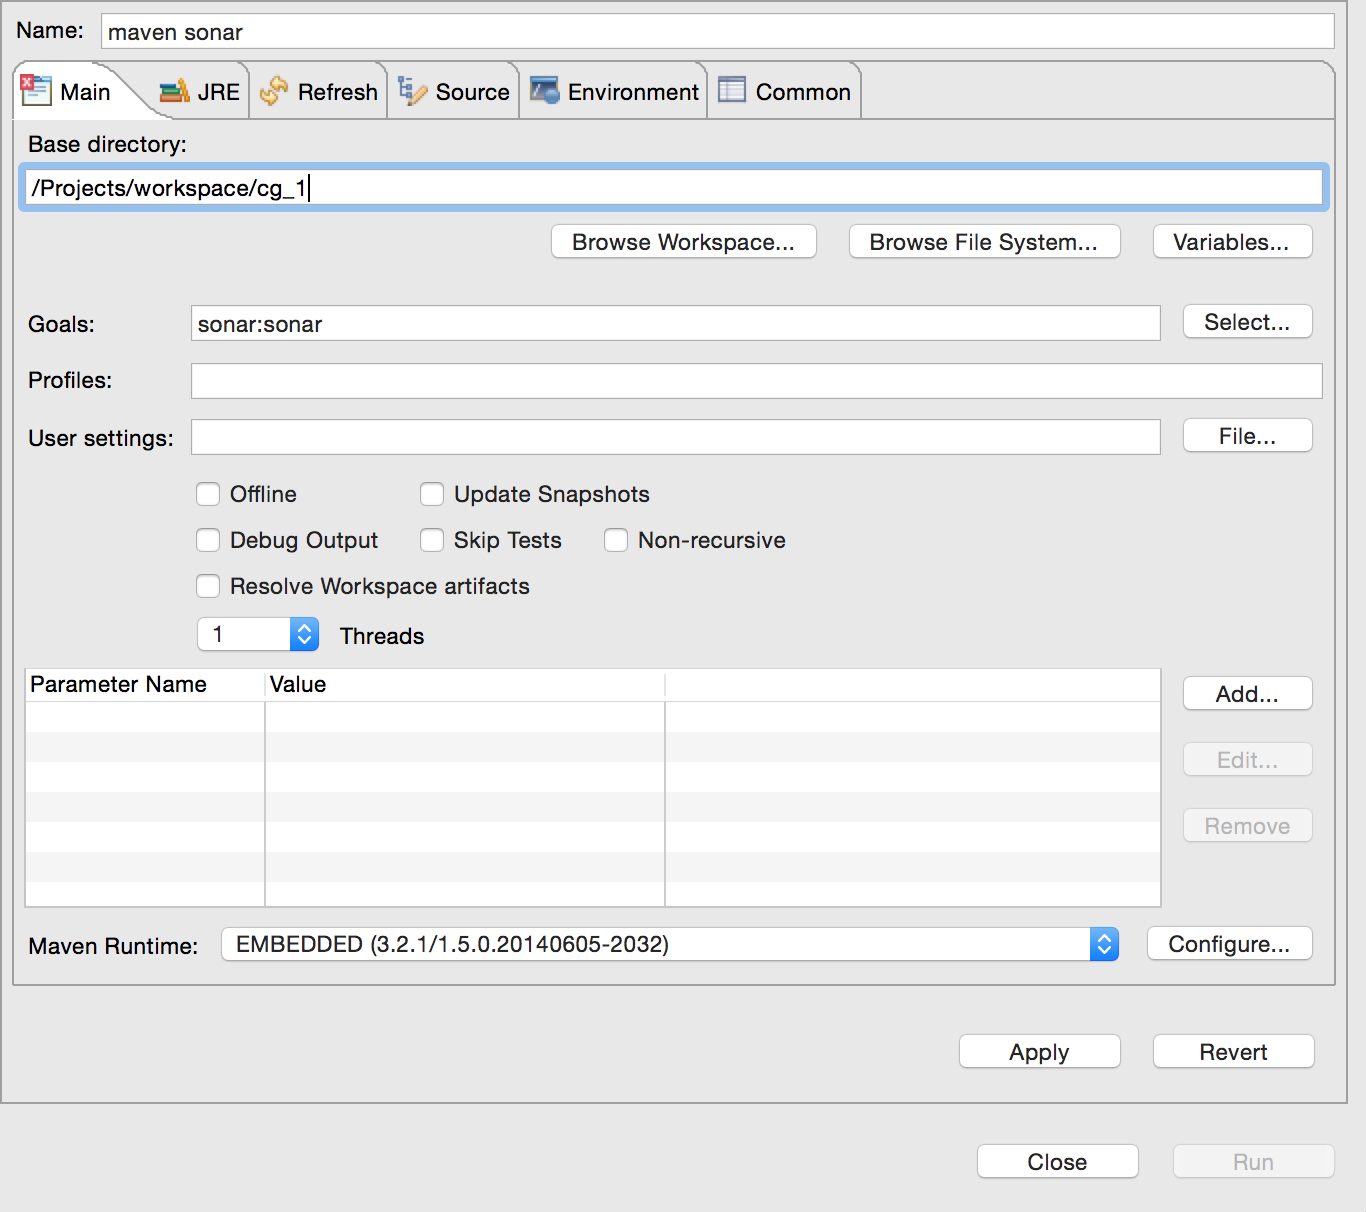
\includegraphics[scale=0.5]{figures/ss5}
\end{center}
\item execute the run configuration
\item access your project in Sonar by going to
  \url{http://localhost:9000/} and see its statistics
\end{itemize}


\subsection{Enable test coverage}
If you notice that the statistics that you option from the previous
sonar analysis does not contain unit test coverage information, you
need to enable test coverage:

\begin{itemize}
\item modify your pom.xml file to include the Jacoco plugin:
\begin{lstlisting}
<plugin>
	<groupId>org.jacoco</groupId>
	<artifactId>jacoco-maven-plugin</artifactId>
	<version>0.5.5.201112152213</version>
	<configuration>
		<destFile>target/jacoco.exec</destFile>
		<dataFile>target/jacoco.exec</dataFile>
	</configuration>
	<executions>
		<execution>
			<id>jacoco-initialize</id>
			<goals>
				<goal>prepare-agent</goal>
			</goals>
		</execution>
		<execution>
			<id>jacoco-site</id>
			<phase>package</phase>
			<goals>
				<goal>report</goal>
			</goals>
		</execution>
	</executions>
</plugin>
\end{lstlisting}
\item Note that, this change is already included in the maven guide

% \item navigate to the root folder of you project
% \item run the following command 
% \begin{lstlisting}
% mvn clean org.jacoco:jacoco-maven-plugin:prepare-agent install
% -Dmaven.test.failure.ignore=true
% \end{lstlisting}
% \item re-run the \texttt{maven sonar} run configuration and go to
%   \url{http://localhost:9000/} to see the code coverage statistics.
\end{itemize}



\subsection{Integrate Sonar with Eclipse}

\begin{itemize}
\item go to Help $>$ Eclipse Marketplace... and search for "SonarQube"
\item check the following features:
\begin{center}
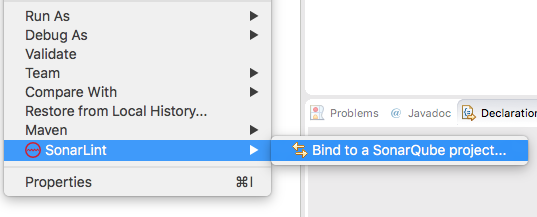
\includegraphics[scale=0.5]{figures/ss6}
\end{center}
\item after the installation open Eclipse $>$ Properties and choose
  SonarQube $>$ Servers.
\item add  \url{http://localhost:9000/} if it is not there
\item add your Sonar credentials (if you haven't changed them the
  default ones are: username = admin and password = admin)
\item save changes
\item right click on the project SonarQube $>$ Analyze
\item you should be able to see Sonar issues tab as well as direct
  Sonar annotations in the code:
\begin{center}
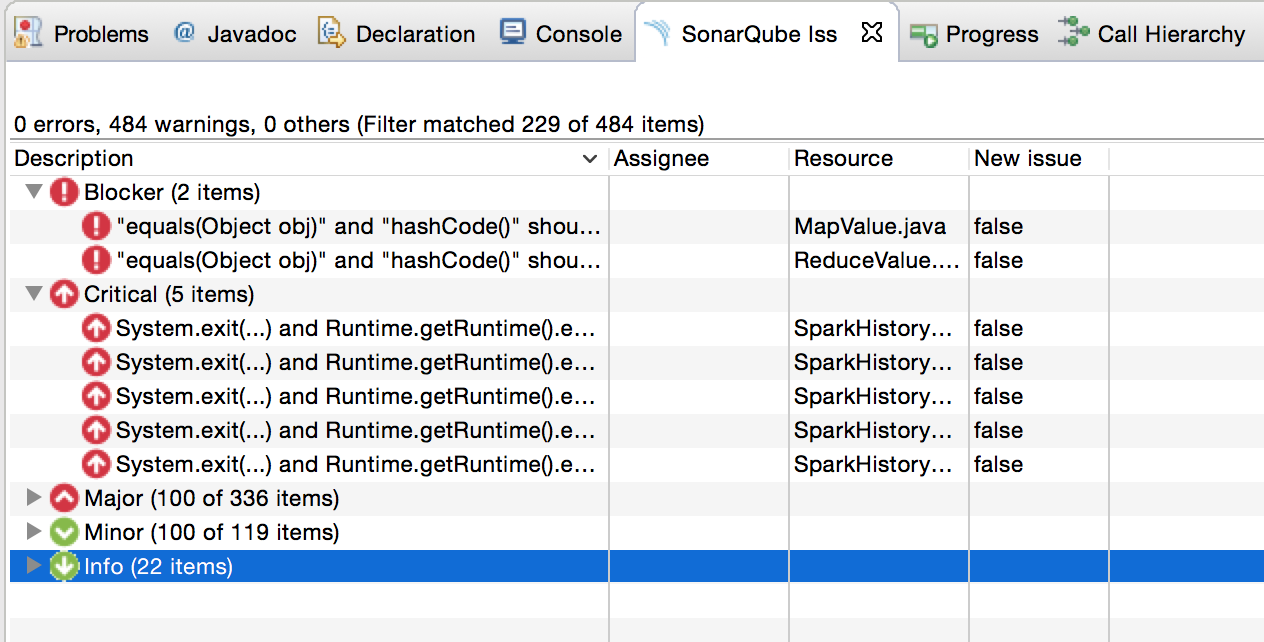
\includegraphics[scale=0.3]{figures/ss7.png}
\end{center}
\item for more details on how to use Sonar, watch the following
  screencast: \url{https://vimeo.com/91781086}
\end{itemize}

\section{Use Sonar}

The home page of SonarQube is called Global Dashboard. It is able to
show multiple projects at once. In your case you will be seeing only
one project, but you are encouraged to use sonar for all the
subsequent projects you develop. Whatever your context, you can
always return to this home page using the "Dashboards" link in the top
left corner of the SonarQube interface. Global Dashboard is highly
configurable and you can add/remove and rearrange the various boxes at
your preference. 
\begin{center}
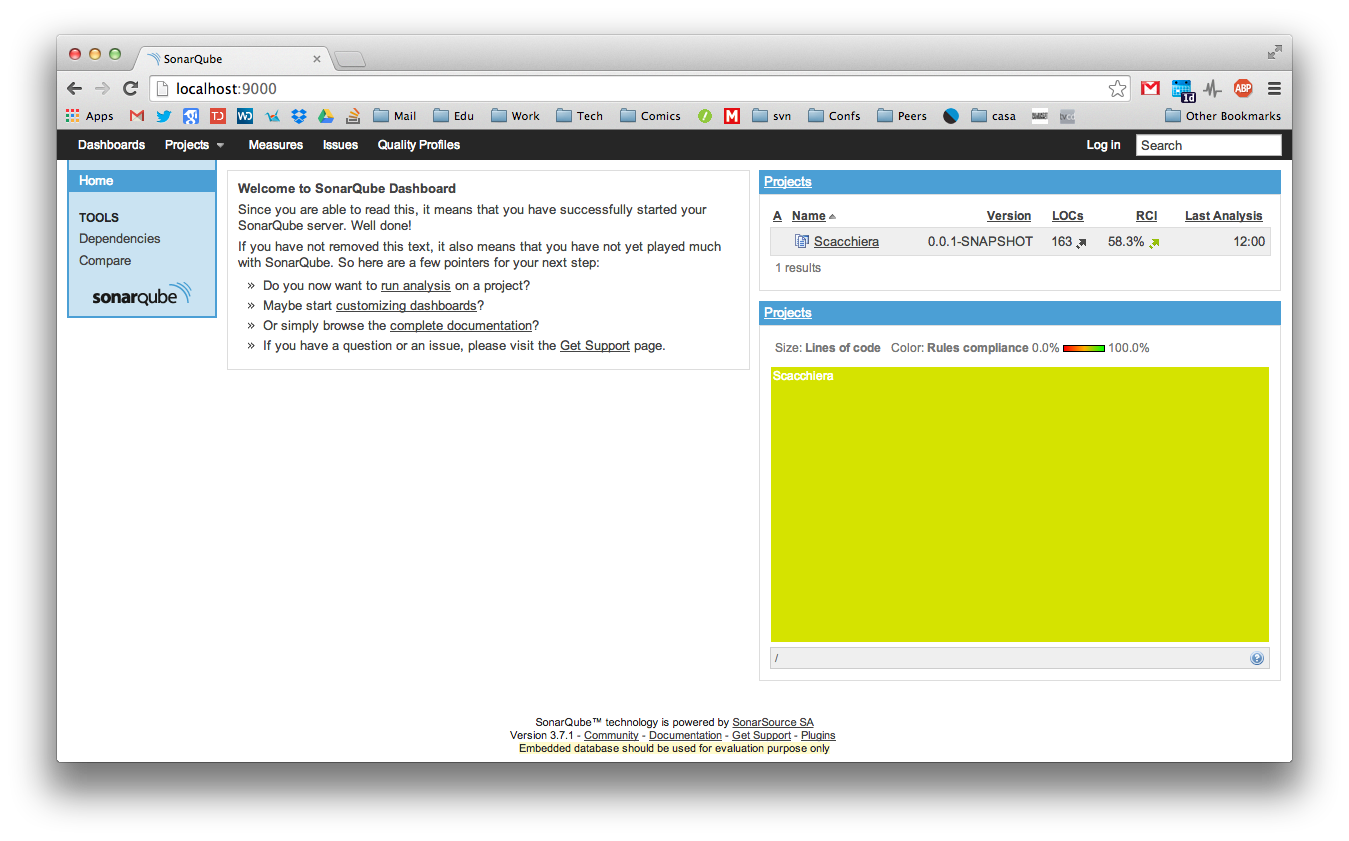
\includegraphics[scale=0.3]{figures/ss1.png}
\end{center}

%SonarQube dashboard

Once you click on a project you will navigate to the Project Dashboard. 
Each box on this page is called a widget. Any widget can be added to a
project dashboard. Thus, any kinds of information from a project or
from the SonarQube instance can be displayed at will, although project
dashboards typically contain only project widgets.
The Default Dashboard gives an overview of your project (with widgets
like Size, etc.) and its quality (with widgets like Issues and
Technical Debt, Duplications, etc.).\footnote{for more details visit: \url{http://docs.sonarqube.org/display/SONAR/Project+Dashboards}}
\begin{center}
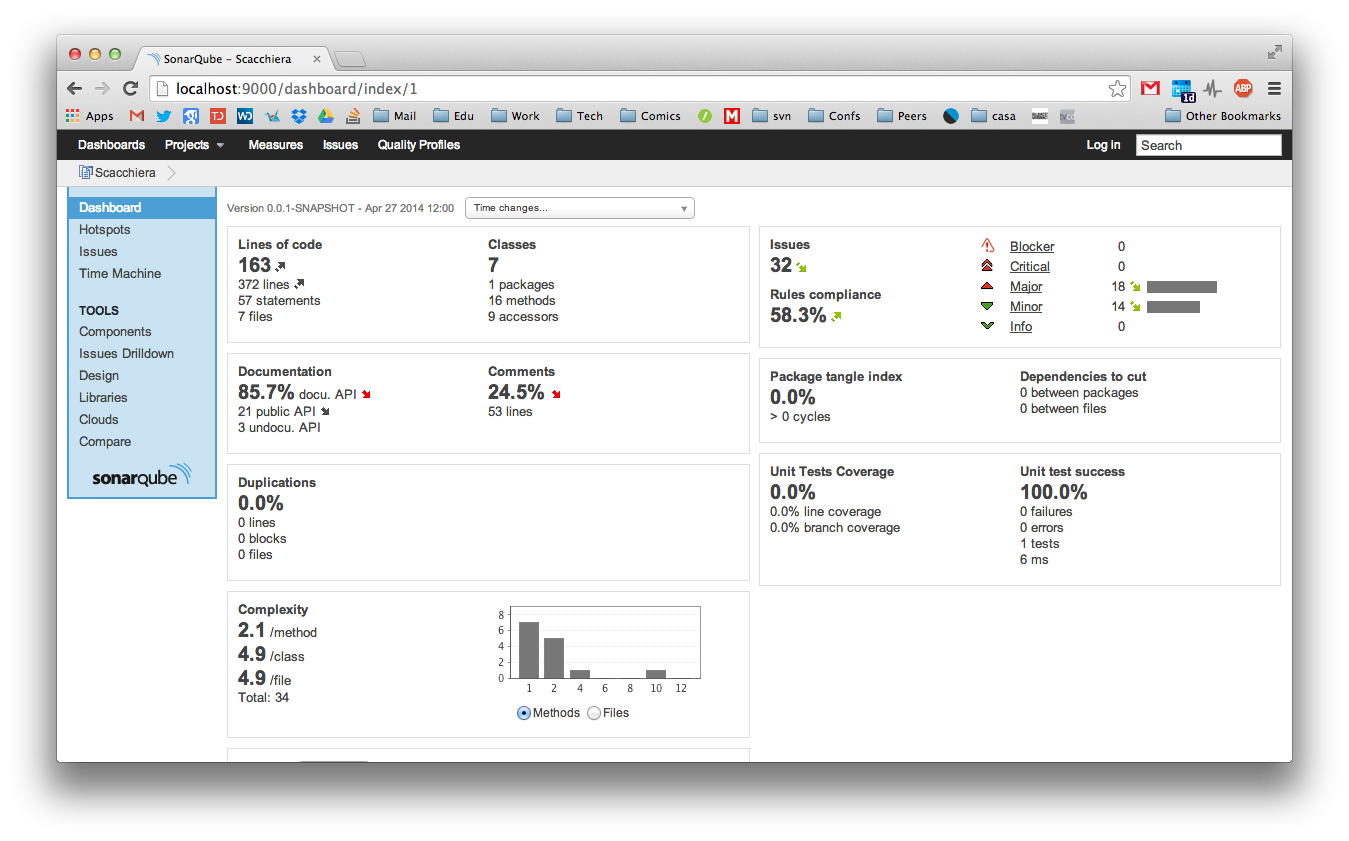
\includegraphics[scale=0.3]{figures/ss2.png}
\end{center}

If you drill down the project issues you can see bugs and potential
bugs discovered by Sonar. They represent things that are going wrong
in your code today or that may go wrong tomorrow. An unconditional
null pointer dereference is a prime example
of a bug. Potential bugs are a bit more subtle, but no less important. 
Typically bugs and potential bugs will show up as Blocker or Critical issues,
although that's fully configurable. 
Sonar will also report any Coding Standards Breaches although
typically at lower severities.
\begin{center}
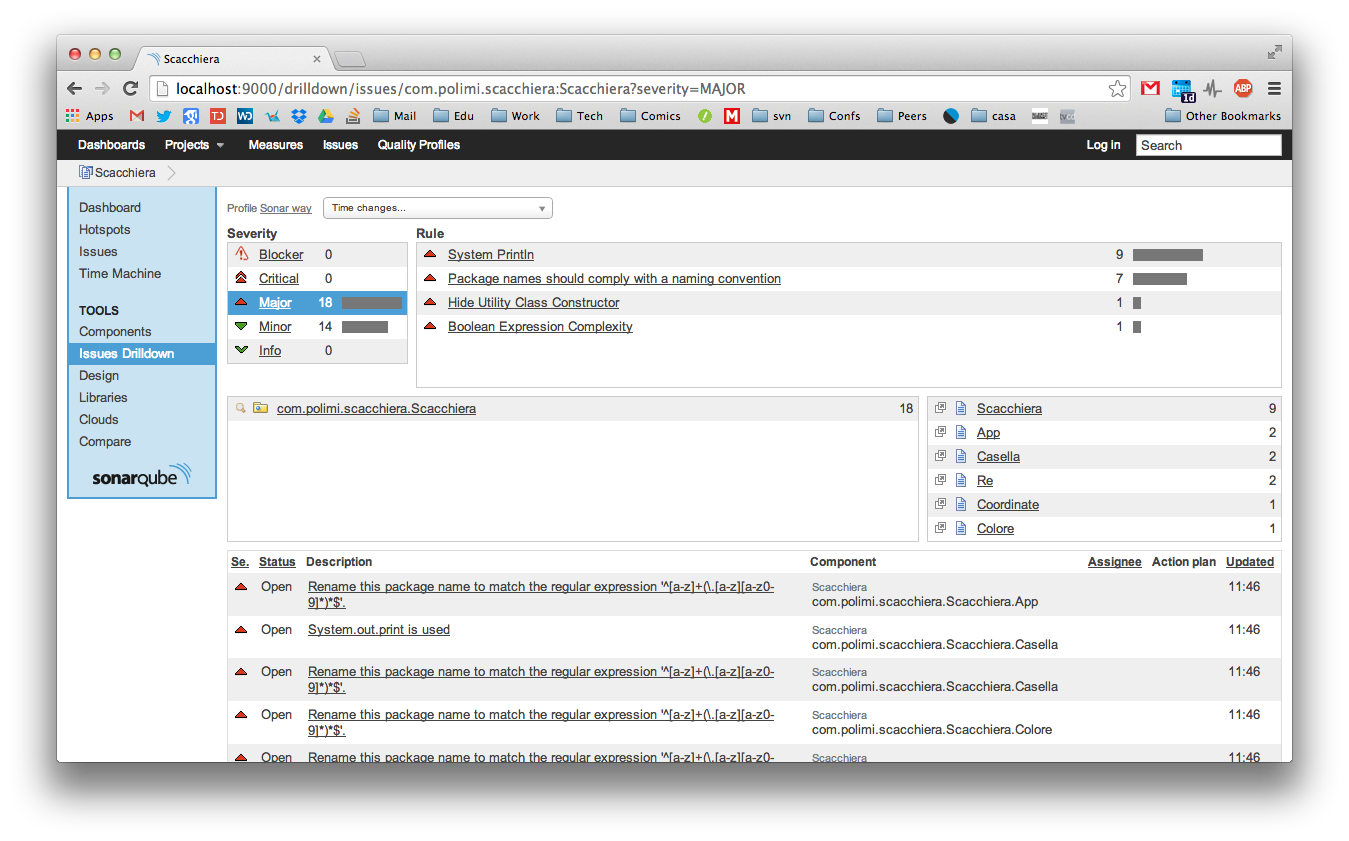
\includegraphics[scale=0.3]{figures/ss3.png}
\end{center}

Every issue will be directly marked in the code, however this is far
more useful if you install the Sonar Eclipse plugin.\footnote{For a
  complete guide to Sonar visit:
\url{http://docs.sonarqube.org/display/SONAR/Documentation}}
\begin{center}
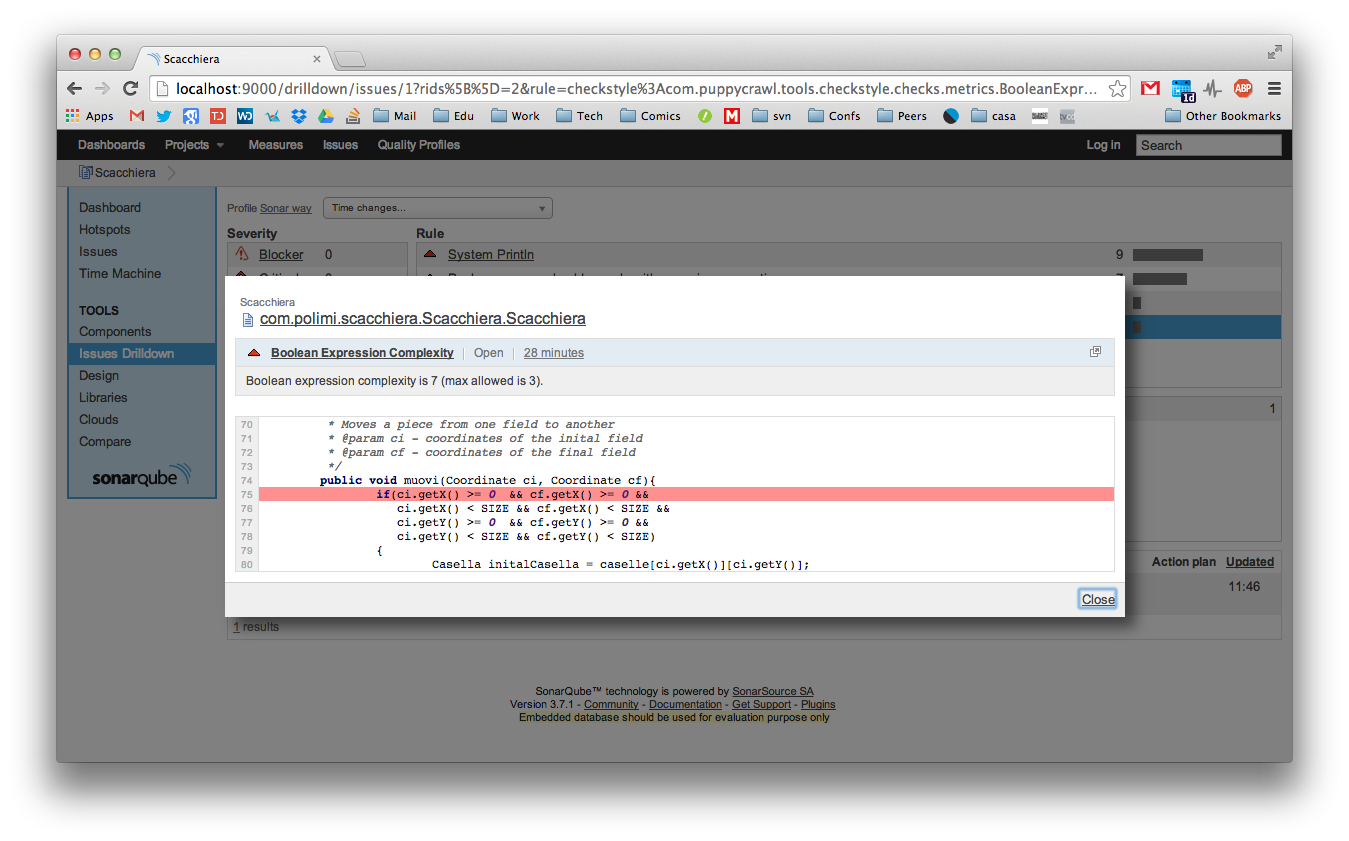
\includegraphics[scale=0.3]{figures/ss4.png}
\end{center}





% \section{Global Sonar}
% \begin{itemize}
% \item ogni gruppo ha un profilo sonar associato al progetto \`e possibile consultare le metriche sonar utilizzando il link \url{http://ing-software.cloudapp.net:9000/} una volta loggati potete analizzare le metriche del vostro progetto.
% \item le credenziali per accedere sono 
% \begin{itemize}
% \item username: matricola
% \item password: changeme
% \end{itemize}
% \item potete modificare le vostre credenziali cliccando sul vostro nome in alto a destra $>$ My profile 
% \end{itemize}



\end{document}

